\documentclass[a4paper]{article}

%================================================================================================================================
%
% Packages
%
%================================================================================================================================

\usepackage[T1]{fontenc} 	% pour caractères accentués
\usepackage[utf8]{inputenc}  % encodage utf8
\usepackage[french]{babel}	% langue : français
\usepackage{fourier}			% caractères plus lisibles
\usepackage[dvipsnames]{xcolor} % couleurs
\usepackage{fancyhdr}		% réglage header footer
\usepackage{needspace}		% empêcher sauts de page mal placés
\usepackage{graphicx}		% pour inclure des graphiques
\usepackage{enumitem,cprotect}		% personnalise les listes d'items (nécessaire pour ol, al ...)
\usepackage{hyperref}		% Liens hypertexte
\usepackage{pstricks,pst-all,pst-node,pstricks-add,pst-math,pst-plot,pst-tree,pst-eucl} % pstricks
\usepackage[a4paper,includeheadfoot,top=2cm,left=3cm, bottom=2cm,right=3cm]{geometry} % marges etc.
\usepackage{comment}			% commentaires multilignes
\usepackage{amsmath,environ} % maths (matrices, etc.)
\usepackage{amssymb,makeidx}
\usepackage{bm}				% bold maths
\usepackage{tabularx}		% tableaux
\usepackage{colortbl}		% tableaux en couleur
\usepackage{fontawesome}		% Fontawesome
\usepackage{environ}			% environment with command
\usepackage{fp}				% calculs pour ps-tricks
\usepackage{multido}			% pour ps tricks
\usepackage[np]{numprint}	% formattage nombre
\usepackage{tikz,tkz-tab} 			% package principal TikZ
\usepackage{pgfplots}   % axes
\usepackage{mathrsfs}    % cursives
\usepackage{calc}			% calcul taille boites
\usepackage[scaled=0.875]{helvet} % font sans serif
\usepackage{svg} % svg
\usepackage{scrextend} % local margin
\usepackage{scratch} %scratch
\usepackage{multicol} % colonnes
%\usepackage{infix-RPN,pst-func} % formule en notation polanaise inversée
\usepackage{listings}

%================================================================================================================================
%
% Réglages de base
%
%================================================================================================================================

\lstset{
language=Python,   % R code
literate=
{á}{{\'a}}1
{à}{{\`a}}1
{ã}{{\~a}}1
{é}{{\'e}}1
{è}{{\`e}}1
{ê}{{\^e}}1
{í}{{\'i}}1
{ó}{{\'o}}1
{õ}{{\~o}}1
{ú}{{\'u}}1
{ü}{{\"u}}1
{ç}{{\c{c}}}1
{~}{{ }}1
}


\definecolor{codegreen}{rgb}{0,0.6,0}
\definecolor{codegray}{rgb}{0.5,0.5,0.5}
\definecolor{codepurple}{rgb}{0.58,0,0.82}
\definecolor{backcolour}{rgb}{0.95,0.95,0.92}

\lstdefinestyle{mystyle}{
    backgroundcolor=\color{backcolour},   
    commentstyle=\color{codegreen},
    keywordstyle=\color{magenta},
    numberstyle=\tiny\color{codegray},
    stringstyle=\color{codepurple},
    basicstyle=\ttfamily\footnotesize,
    breakatwhitespace=false,         
    breaklines=true,                 
    captionpos=b,                    
    keepspaces=true,                 
    numbers=left,                    
xleftmargin=2em,
framexleftmargin=2em,            
    showspaces=false,                
    showstringspaces=false,
    showtabs=false,                  
    tabsize=2,
    upquote=true
}

\lstset{style=mystyle}


\lstset{style=mystyle}
\newcommand{\imgdir}{C:/laragon/www/newmc/assets/imgsvg/}
\newcommand{\imgsvgdir}{C:/laragon/www/newmc/assets/imgsvg/}

\definecolor{mcgris}{RGB}{220, 220, 220}% ancien~; pour compatibilité
\definecolor{mcbleu}{RGB}{52, 152, 219}
\definecolor{mcvert}{RGB}{125, 194, 70}
\definecolor{mcmauve}{RGB}{154, 0, 215}
\definecolor{mcorange}{RGB}{255, 96, 0}
\definecolor{mcturquoise}{RGB}{0, 153, 153}
\definecolor{mcrouge}{RGB}{255, 0, 0}
\definecolor{mclightvert}{RGB}{205, 234, 190}

\definecolor{gris}{RGB}{220, 220, 220}
\definecolor{bleu}{RGB}{52, 152, 219}
\definecolor{vert}{RGB}{125, 194, 70}
\definecolor{mauve}{RGB}{154, 0, 215}
\definecolor{orange}{RGB}{255, 96, 0}
\definecolor{turquoise}{RGB}{0, 153, 153}
\definecolor{rouge}{RGB}{255, 0, 0}
\definecolor{lightvert}{RGB}{205, 234, 190}
\setitemize[0]{label=\color{lightvert}  $\bullet$}

\pagestyle{fancy}
\renewcommand{\headrulewidth}{0.2pt}
\fancyhead[L]{maths-cours.fr}
\fancyhead[R]{\thepage}
\renewcommand{\footrulewidth}{0.2pt}
\fancyfoot[C]{}

\newcolumntype{C}{>{\centering\arraybackslash}X}
\newcolumntype{s}{>{\hsize=.35\hsize\arraybackslash}X}

\setlength{\parindent}{0pt}		 
\setlength{\parskip}{3mm}
\setlength{\headheight}{1cm}

\def\ebook{ebook}
\def\book{book}
\def\web{web}
\def\type{web}

\newcommand{\vect}[1]{\overrightarrow{\,\mathstrut#1\,}}

\def\Oij{$\left(\text{O}~;~\vect{\imath},~\vect{\jmath}\right)$}
\def\Oijk{$\left(\text{O}~;~\vect{\imath},~\vect{\jmath},~\vect{k}\right)$}
\def\Ouv{$\left(\text{O}~;~\vect{u},~\vect{v}\right)$}

\hypersetup{breaklinks=true, colorlinks = true, linkcolor = OliveGreen, urlcolor = OliveGreen, citecolor = OliveGreen, pdfauthor={Didier BONNEL - https://www.maths-cours.fr} } % supprime les bordures autour des liens

\renewcommand{\arg}[0]{\text{arg}}

\everymath{\displaystyle}

%================================================================================================================================
%
% Macros - Commandes
%
%================================================================================================================================

\newcommand\meta[2]{    			% Utilisé pour créer le post HTML.
	\def\titre{titre}
	\def\url{url}
	\def\arg{#1}
	\ifx\titre\arg
		\newcommand\maintitle{#2}
		\fancyhead[L]{#2}
		{\Large\sffamily \MakeUppercase{#2}}
		\vspace{1mm}\textcolor{mcvert}{\hrule}
	\fi 
	\ifx\url\arg
		\fancyfoot[L]{\href{https://www.maths-cours.fr#2}{\black \footnotesize{https://www.maths-cours.fr#2}}}
	\fi 
}


\newcommand\TitreC[1]{    		% Titre centré
     \needspace{3\baselineskip}
     \begin{center}\textbf{#1}\end{center}
}

\newcommand\newpar{    		% paragraphe
     \par
}

\newcommand\nosp {    		% commande vide (pas d'espace)
}
\newcommand{\id}[1]{} %ignore

\newcommand\boite[2]{				% Boite simple sans titre
	\vspace{5mm}
	\setlength{\fboxrule}{0.2mm}
	\setlength{\fboxsep}{5mm}	
	\fcolorbox{#1}{#1!3}{\makebox[\linewidth-2\fboxrule-2\fboxsep]{
  		\begin{minipage}[t]{\linewidth-2\fboxrule-4\fboxsep}\setlength{\parskip}{3mm}
  			 #2
  		\end{minipage}
	}}
	\vspace{5mm}
}

\newcommand\CBox[4]{				% Boites
	\vspace{5mm}
	\setlength{\fboxrule}{0.2mm}
	\setlength{\fboxsep}{5mm}
	
	\fcolorbox{#1}{#1!3}{\makebox[\linewidth-2\fboxrule-2\fboxsep]{
		\begin{minipage}[t]{1cm}\setlength{\parskip}{3mm}
	  		\textcolor{#1}{\LARGE{#2}}    
 	 	\end{minipage}  
  		\begin{minipage}[t]{\linewidth-2\fboxrule-4\fboxsep}\setlength{\parskip}{3mm}
			\raisebox{1.2mm}{\normalsize\sffamily{\textcolor{#1}{#3}}}						
  			 #4
  		\end{minipage}
	}}
	\vspace{5mm}
}

\newcommand\cadre[3]{				% Boites convertible html
	\par
	\vspace{2mm}
	\setlength{\fboxrule}{0.1mm}
	\setlength{\fboxsep}{5mm}
	\fcolorbox{#1}{white}{\makebox[\linewidth-2\fboxrule-2\fboxsep]{
  		\begin{minipage}[t]{\linewidth-2\fboxrule-4\fboxsep}\setlength{\parskip}{3mm}
			\raisebox{-2.5mm}{\sffamily \small{\textcolor{#1}{\MakeUppercase{#2}}}}		
			\par		
  			 #3
 	 		\end{minipage}
	}}
		\vspace{2mm}
	\par
}

\newcommand\bloc[3]{				% Boites convertible html sans bordure
     \needspace{2\baselineskip}
     {\sffamily \small{\textcolor{#1}{\MakeUppercase{#2}}}}    
		\par		
  			 #3
		\par
}

\newcommand\CHelp[1]{
     \CBox{Plum}{\faInfoCircle}{À RETENIR}{#1}
}

\newcommand\CUp[1]{
     \CBox{NavyBlue}{\faThumbsOUp}{EN PRATIQUE}{#1}
}

\newcommand\CInfo[1]{
     \CBox{Sepia}{\faArrowCircleRight}{REMARQUE}{#1}
}

\newcommand\CRedac[1]{
     \CBox{PineGreen}{\faEdit}{BIEN R\'EDIGER}{#1}
}

\newcommand\CError[1]{
     \CBox{Red}{\faExclamationTriangle}{ATTENTION}{#1}
}

\newcommand\TitreExo[2]{
\needspace{4\baselineskip}
 {\sffamily\large EXERCICE #1\ (\emph{#2 points})}
\vspace{5mm}
}

\newcommand\img[2]{
          \includegraphics[width=#2\paperwidth]{\imgdir#1}
}

\newcommand\imgsvg[2]{
       \begin{center}   \includegraphics[width=#2\paperwidth]{\imgsvgdir#1} \end{center}
}


\newcommand\Lien[2]{
     \href{#1}{#2 \tiny \faExternalLink}
}
\newcommand\mcLien[2]{
     \href{https~://www.maths-cours.fr/#1}{#2 \tiny \faExternalLink}
}

\newcommand{\euro}{\eurologo{}}

%================================================================================================================================
%
% Macros - Environement
%
%================================================================================================================================

\newenvironment{tex}{ %
}
{%
}

\newenvironment{indente}{ %
	\setlength\parindent{10mm}
}

{
	\setlength\parindent{0mm}
}

\newenvironment{corrige}{%
     \needspace{3\baselineskip}
     \medskip
     \textbf{\textsc{Corrigé}}
     \medskip
}
{
}

\newenvironment{extern}{%
     \begin{center}
     }
     {
     \end{center}
}

\NewEnviron{code}{%
	\par
     \boite{gray}{\texttt{%
     \BODY
     }}
     \par
}

\newenvironment{vbloc}{% boite sans cadre empeche saut de page
     \begin{minipage}[t]{\linewidth}
     }
     {
     \end{minipage}
}
\NewEnviron{h2}{%
    \needspace{3\baselineskip}
    \vspace{0.6cm}
	\noindent \MakeUppercase{\sffamily \large \BODY}
	\vspace{1mm}\textcolor{mcgris}{\hrule}\vspace{0.4cm}
	\par
}{}

\NewEnviron{h3}{%
    \needspace{3\baselineskip}
	\vspace{5mm}
	\textsc{\BODY}
	\par
}

\NewEnviron{margeneg}{ %
\begin{addmargin}[-1cm]{0cm}
\BODY
\end{addmargin}
}

\NewEnviron{html}{%
}

\begin{document}
\meta{url}{/exercices/qcm-bac-blanc-es-l-sujet-1-maths-cours-2017/}
\meta{pid}{10381}
\meta{titre}{QCM - Bac blanc ES/L Sujet 1 - Maths-cours 2017}
\meta{type}{exercices}
%
\begin{h2}Exercice 1 (5 points)\end{h2}
\par
\emph{Cet exercice est un QCM (questionnaire à choix multiples). Pour chacune des questions suivantes, une seule des réponses proposées est exacte. \\Indiquer sur la copie le numéro de la question et la réponse choisie en justifiant le choix effectué. }
\par
\medskip
\par
\emph{\textbf{Une réponse non justifiée ne sera pas prise en compte.}}
\par
Pour les questions \textbf{1.}, \textbf{2.} et \textbf{3.}, $f$ est une fonction définie et dérivable sur l'intervalle $[-4~;~2]$ dont la courbe représentative $\mathscr{C}_{f}$, dans un repère orthogonal, est tracée ci-après.
\par
\begin{center}
     \begin{extern}%width="600" alt=""
          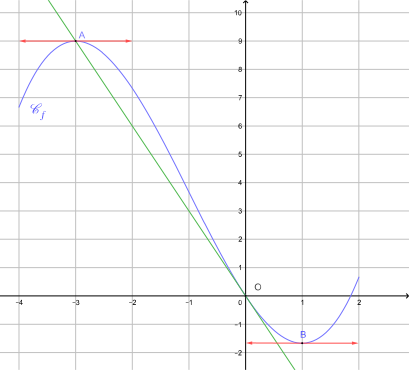
\includegraphics[width=0.9\textwidth]{images/BBESL-s1-1-1}% gbb 1 unite=2cm
     \end{extern}
\end{center}
\par
La courbe $\mathscr{C}_{f}$ passe par l'origine $O$ du repère et par les points $A(-3~;~9)$ et $B\left(1~;~-\dfrac{5}{3}\right)$.
\par
Les tangentes à la courbe $\mathscr{C}_{f}$ aux points $A$ et $B$ sont parallèles à l'axe des abscisses.
\par
La tangente à la courbe $\mathscr{C}_{f}$ au point $O$ passe par le point $A$.
\par
\medskip
\par
On note $f^{\prime}$  la fonction dérivée de la fonction $f$.
\par
\begin{itemize}
     \needspace{4\baselineskip}
     \item \textbf{Question 1 :}
     \par
     La valeur exacte de $f(0)$ est :
     \par
     \textbf{a.~~} $0$ \\
     \textbf{b.~~} $1$ \\
     \textbf{c.~~} $-\dfrac{5}{3}$ \\
     \textbf{d.~~} autre réponse \\
     \par
     \needspace{4\baselineskip}
     \item \textbf{Question 2 :}
     \par
     La valeur exacte de $f'(0)$ est :
     \par
     \textbf{a.~~} $0$ \\
     \textbf{b.~~} $-3$ \\
     \textbf{c.~~} $3$ \\
     \textbf{d.~~} autre réponse \\
     \par
     \needspace{4\baselineskip}
     \item \textbf{Question 3 :}
     \par
     L'ensemble $S$ des solutions de l'équation $f'(x)=0$ est :
     \par
     \textbf{a.~~} $S=\emptyset$ \\
     \textbf{b.~~} $S=\left\{0\right\}$  \\
     \textbf{c.~~} $S=\left\{-3~;~1\right\}$ \\
     \textbf{d.~~} $S=\left\{-\dfrac{5}{3}~;~9\right\}$ \\
     \par
     \needspace{4\baselineskip}
     \item \textbf{Question 4 :}
     \par
     Lors des soldes d'hiver, le prix d'un article est passé de 150~euros à 120~euros.
     \par
     Quel est le taux de la remise accordée par le vendeur ?
     \par
     \textbf{a.~~} 15\% \\
     \textbf{b.~~} 20\%  \\
     \textbf{c.~~} 25\% \\
     \textbf{d.~~} 30\% \\
     \par
     \needspace{4\baselineskip}
     \item \textbf{Question 5 :}
     \par
     De 2005 à 2010, la population d'une ville a augmenté de 5\% puis, de 2010 à 2015, a diminué de 3\%.
     \par
     Le taux d'évolution global de cette population entre 2005 et 2015 est :
     \par
     \textbf{a.~~} 2\% \\
     \textbf{b.~~} 8,15\%  \\
     \textbf{c.~~} 1,85\% \\
     \textbf{d.~~} 0,2\% \\
     \par
\end{itemize}
\begin{corrige}
     \begin{itemize}
          \item \textbf{Question 1 :}
          \par
          Réponse correcte :\quad\textbf{ a.}
          \par
          La courbe $\mathscr{C}_f$ passe par l'origine donc $f(0)=0$.
          \par
          \cadre{rouge}{À retenir}{
               \par
               Soient $\mathscr{C}_f$ la courbe représentative d'une fonction $f$ et $M$ un point de coordonnées $\left(x_M~;~y_M\right)$.
               \par
               Le point $M$ appartient à la courbe $\mathscr{C}_f$ si et seulement si ${f\left(x_M\right)=y_M}$.
               \par
               \textit{Ici, le point $O(0~;~0)$ appartient à la courbe $\mathscr{C}_f$ donc ${f(0)=0}$.}
          }
          \par
          \item \textbf{Question 2 :}
          \par
          Réponse correcte :\quad\textbf{ b.}
          \par
          $f'(0)$ est le coefficient directeur de la tangente en $O$ à la courbe $\mathscr{C}_f$.
          \par
          Cette tangente est la droite $(OA)$ donc :
          \[ f'(0)=\dfrac{y_A-y_O}{x_A-x_O}=\dfrac{9}{-3}=-3.\]
          \par
          \cadre{rouge}{À retenir}{
               $f'(a)$ est le \textbf{coefficient directeur de la tangente} au point de la courbe $\mathscr{C}_f$ d'\textbf{abscisse} $a$.
          }
          \par
          \vspace{-8mm}
          \par
          \cadre{rouge}{À retenir}{
               Soient $A$ et $B$ deux points de coordonnées respectives $\left(x_A~;~y_A\right)$ et $\left(x_B~;~y_B\right)$.
               \par
               Le \textbf{coefficient directeur} de la droite $(AB)$ est :
               \[ a = \dfrac{y_B-y_A}{x_B-x_A}.\]
               \par
          }
          \par
          \item \textbf{Question 3 :}
          \par
          Réponse correcte :\quad\textbf{ c.}
          \par
          $f'(x)=0$ si et seulement si la tangente à la courbe $\mathscr{C}_f$ au point d'abscisse $x$ est parallèle à l'axe des abscisses.
          \par
          D'après l'énoncé, ceci se produit aux points $A$ et $B$ d'abscisses respectives $-3$ et $1$.
          \par
          \cadre{rouge}{À retenir}{
               \par
               $f'(a)=0$ si et seulement si la tangente à la courbe représentative de $f$ au point d'abscisse $a$ est \textbf{parallèle à l'axe des abscisses}.
          }
          \par
          \item \textbf{Question 4 :}
          \par
          Réponse correcte :\quad\textbf{ b.}
          \par
          Le taux d'évolution faisant passer de 150 à 120 est :
          \par
          $t=\dfrac{120-150}{150}=-\dfrac{30}{150}=-0,2=-\dfrac{20}{100}=-20\%$.
          \par
          Le taux de la remise effectuée par le vendeur est 20\%.
          \par
          \cadre{rouge}{À retenir}{
               \par
               Lorsqu'une valeur passe de $V_0$ à $V_1$, le taux d'évolution est :
               \[ t = \dfrac{V_1-V_0}{V_0}. \]
          }
          \par
          \item \textbf{Question 5 :}
          \par
          Réponse correcte :\quad\textbf{ c.}
          \par
          Une augmentation de $5\%$ correspond à un coefficient multiplicateur :
          \[ CM_1=1+\dfrac{5}{100} = 1,05.\]
          \par
          Une diminution de $3\%$ correspond à un coefficient multiplicateur :
          \[ CM_2=1-\dfrac{3}{100} =0,97. \]
          \par
          Le coefficient multiplicateur global $CM_g$ est :
          \par
          $ CM_g=CM_1\times CM_2 = 1,05\times 0,97 = 1,0185 = 1+\dfrac{1,85}{100}. $
          \par
          Le taux d'évolution global de la population entre 2005 et 2015 est $1,85\%$.
          \par
          \cadre{rouge}{À retenir}{
               \par
               Lorsqu'une valeur subit plusieurs variations successives, \textbf{le coefficient multiplicateur global est égal au produit des coefficients multiplicateurs} associés à chaque évolution.
          }
          \par
     \end{itemize}
     \par
\end{corrige}

\end{document}